\documentclass{article}
\usepackage{titlesec}
\usepackage[a4paper, left=1in, right=1in, bottom=0.4in, top=0.4in]{geometry}
\usepackage{tikz}
\usetikzlibrary{shapes.geometric, arrows}
\tikzstyle{startstop} = [rectangle, rounded corners, minimum width=3cm, minimum height=1cm,text centered, draw=black, fill=red!30]
\tikzstyle{process} = [rectangle, minimum width=3cm, minimum height=1cm, text centered, draw=black, fill=blue!30]
\tikzstyle{decision} = [diamond, minimum width=3cm, minimum height=1cm, text centered, draw=black, fill=yellow!30]
\tikzstyle{arrow} = [thick,->,>=stealth]

\titleformat{\section}{\Large\bfseries}{\thesection.}{0.5em}{}
\titleformat{\subsection}{\large\bfseries}{\thesubsection.}{0.5em}{}

\begin{document}

\section{User Definition}
A user is a person who enters the app to access services such as searching for nearby clinics and doctors. They do not need special registration and can easily access information.

\subsection{Main Tasks of User}
\begin{itemize}
    \item \textbf{Find nearby clinics} and view their locations.
    \item \textbf{Find available doctors} and check their specialties.
    \item \textbf{View schedules} of clinics and doctors.
    \item \textbf{Get contact numbers} to call clinics or book an appointment.
\end{itemize}

% TODO: User Diagram
\subsection{User Diagram}
\vspace{0.5cm}

\begin{center}
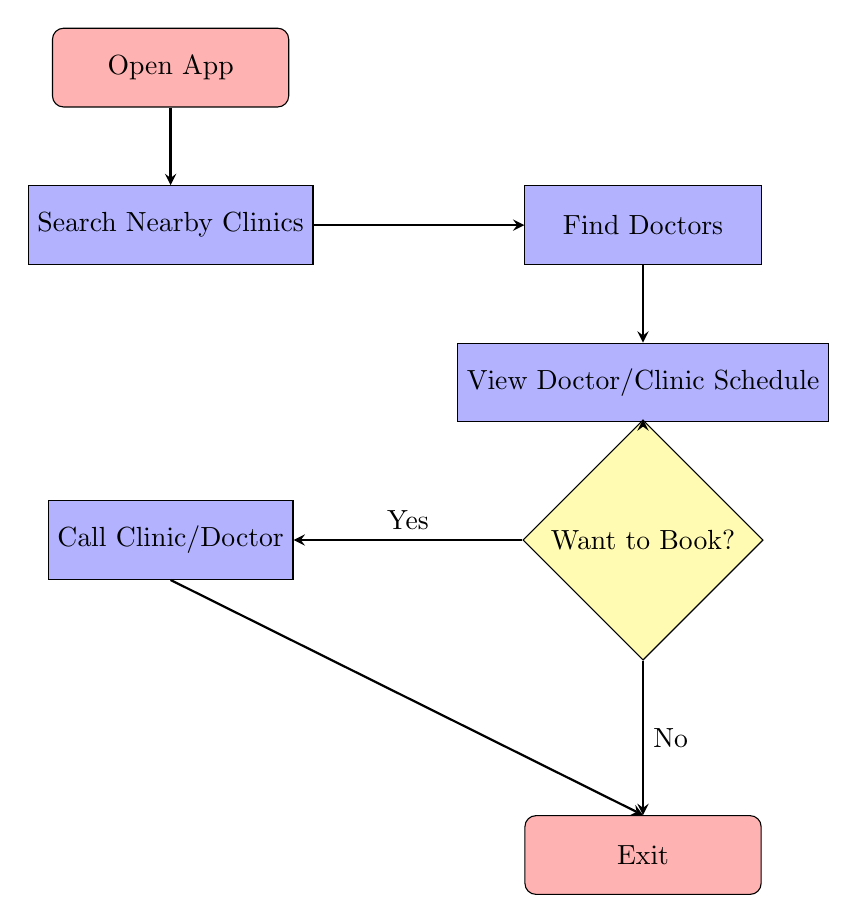
\begin{tikzpicture}[node distance=2cm]

    \node (start) [startstop] {Open App};
    \node (searchClinic) [process, below of=start] {Search Nearby Clinics};
    \node (searchDoctor) [process, right of=searchClinic, xshift=4cm] {Find Doctors};
    \node (viewSchedule) [process, below of=searchDoctor] {View Doctor/Clinic Schedule};
    \node (book) [decision, below of=viewSchedule] {Want to Book?};
    \node (call) [process, left of=book, xshift=-4cm] {Call Clinic/Doctor};
    \node (exit) [startstop, below of=book, yshift=-2cm] {Exit};

    \draw [arrow] (start) -- (searchClinic);
    \draw [arrow] (searchClinic.east) -- (searchDoctor.west);
    \draw [arrow] (searchDoctor) -- (viewSchedule);
    \draw [arrow] (viewSchedule) -- (book);
    \draw [arrow] (book.south) -- node[anchor=west] {No} (exit.north);
    \draw [arrow] (book.west) -- node[anchor=south] {Yes} (call.east);
    \draw [arrow] (call.south) -- (exit.north);

\end{tikzpicture}
\end{center}

\section{Clinic Definition}
A clinic is an entity that registers in the app to add doctors and manage their data. When a clinic registers, it is not accepted automatically; it requires approval from the admin.

\subsection{Main Task of the Clinic}
\begin{itemize}
    \item Enter clinic information during registration (name, address, phone number, specialties).
    \item Wait for \textbf{admin approval} before becoming active.
    \item Once approved, the clinic can:
    \begin{itemize}
        \item \textbf{Add doctors} to the system.
        \item \textbf{Provide login credentials} (email and password) to doctors.
    \end{itemize}
\end{itemize}

%TODO: Clinic Diagram 

\subsection{Clinic Diagram}

\begin{center}
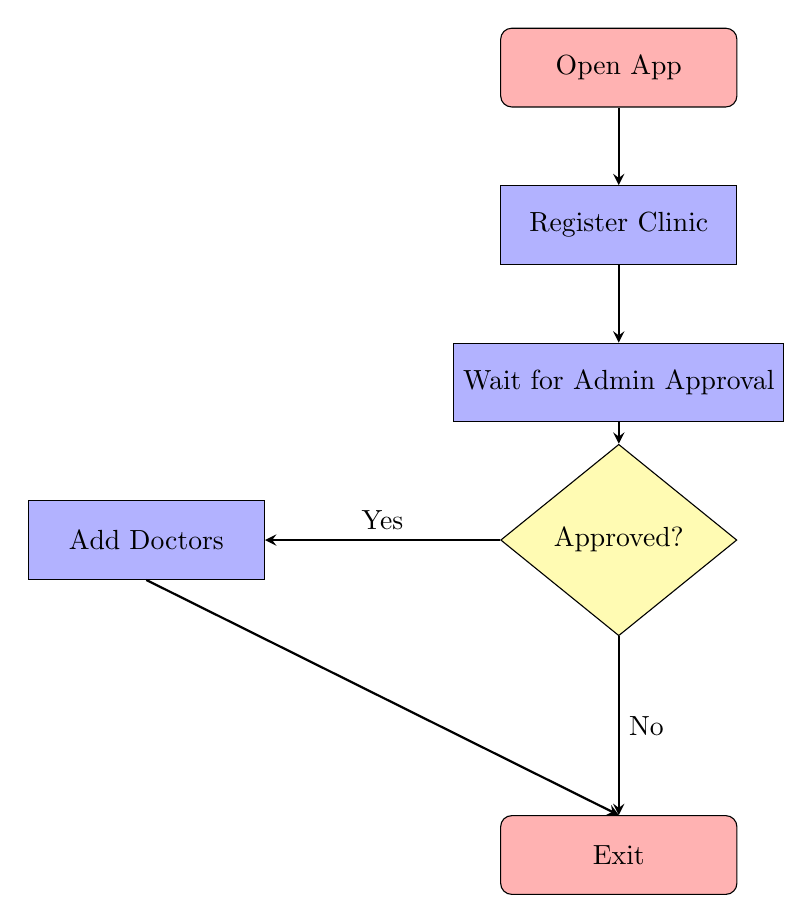
\begin{tikzpicture}[node distance=2cm]

    \node (start) [startstop] {Open App};
    \node (register) [process, below of=start] {Register Clinic};
    \node (wait) [process, below of=register] {Wait for Admin Approval};
    \node (approved) [decision, below of=wait] {Approved?};
    \node (addDoctors) [process, left of=approved, xshift=-4cm] {Add Doctors};
    \node (exit) [startstop, below of=approved, yshift=-2cm] {Exit};

    \draw [arrow] (start) -- (register);
    \draw [arrow] (register) -- (wait);
    \draw [arrow] (wait) -- (approved);
    \draw [arrow] (approved.west) -- node[anchor=south] {Yes} (addDoctors.east);
    \draw [arrow] (addDoctors.south) -- (exit.north);
    \draw [arrow] (approved.south) -- node[anchor=west] {No} (exit.north);

\end{tikzpicture}
\end{center}

\section{Doctor Definition}
A doctor is a user who receives login credentials from the clinic they work at. Doctors cannot register independently.

\subsection{Doctor Tasks}
\begin{itemize}
    \item Log in using \textbf{the email and password} provided by the clinic.
    \item Access and manage \textbf{their schedule}.
    \item Receive \textbf{patient bookings} and view appointment details.
\end{itemize}

% TODO: Doctor Diagram

\subsection{Doctor Diagram}

\begin{center}
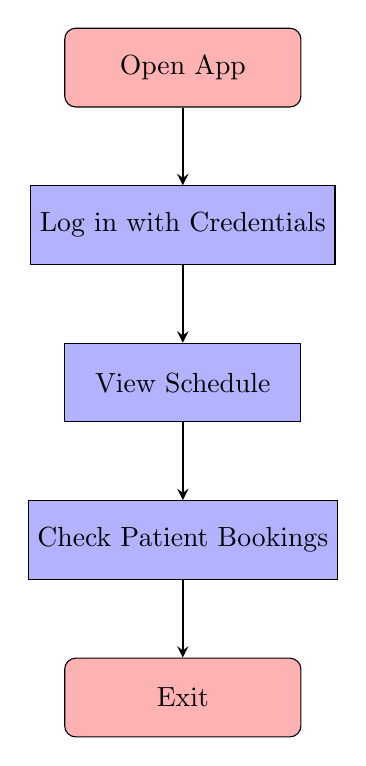
\begin{tikzpicture}[node distance=2cm]

    \node (start) [startstop] {Open App};
    \node (login) [process, below of=start] {Log in with Credentials};
    \node (viewSchedule) [process, below of=login] {View Schedule};
    \node (appointments) [process, below of=viewSchedule] {Check Patient Bookings};
    \node (exit) [startstop, below of=appointments] {Exit};

    \draw [arrow] (start) -- (login);
    \draw [arrow] (login) -- (viewSchedule);
    \draw [arrow] (viewSchedule) -- (appointments);
    \draw [arrow] (appointments) -- (exit);

\end{tikzpicture}
\end{center}
\section{Admin Definition}
The admin is responsible for accepting or rejecting newly registered clinics. They have a separate application to manage the system.

\subsection{Admin Tasks}
\begin{itemize}
    \item Review \textbf{new clinic registration requests}.
    \item Accept or reject clinics based on the provided information.
    \item Ensure the smooth operation of the platform.
\end{itemize}

% TODO: Admin Diagram

\subsection{Admin Diagram}

\begin{center}
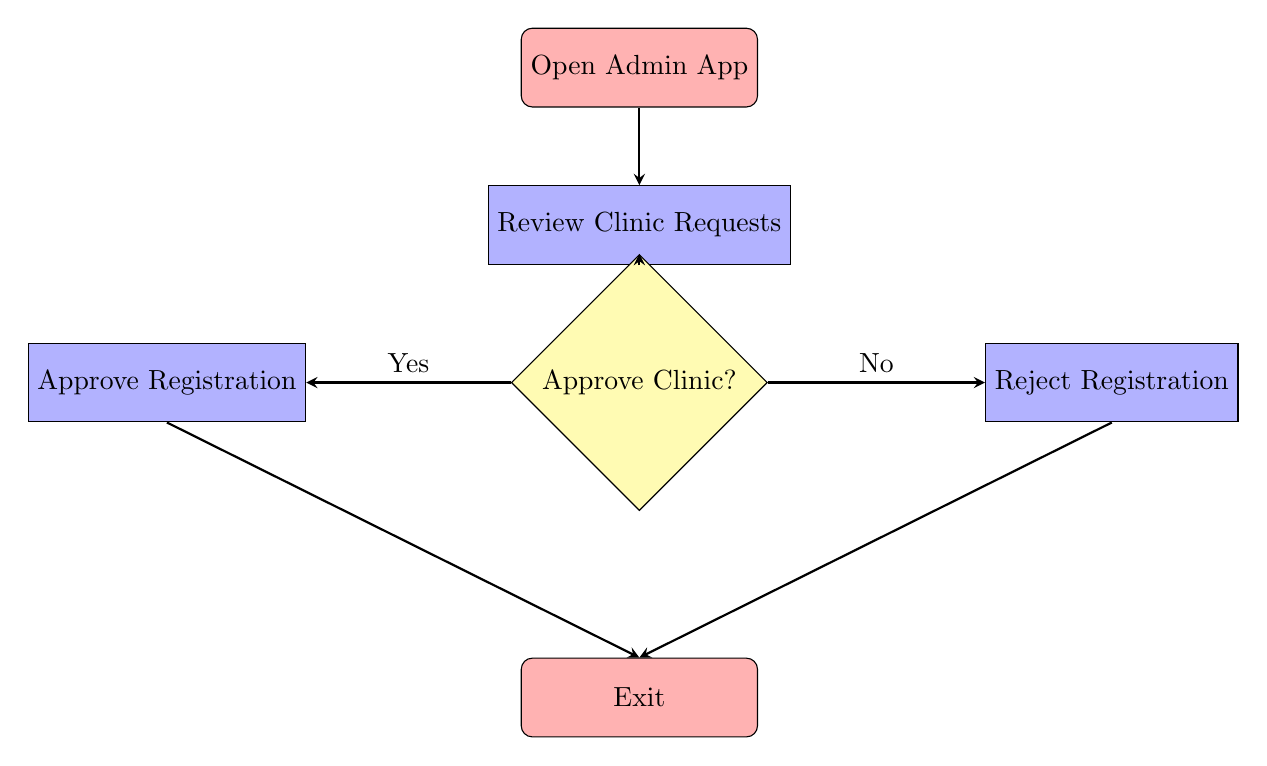
\begin{tikzpicture}[node distance=2cm]

    \node (start) [startstop] {Open Admin App};
    \node (review) [process, below of=start] {Review Clinic Requests};
    \node (approve) [decision, below of=review] {Approve Clinic?};
    \node (approveAction) [process, left of=approve, xshift=-4cm] {Approve Registration};
    \node (rejectAction) [process, right of=approve, xshift=4cm] {Reject Registration};
    \node (exit) [startstop, below of=approve, yshift=-2cm] {Exit};

    \draw [arrow] (start) -- (review);
    \draw [arrow] (review) -- (approve);
    \draw [arrow] (approve.west) -- node[anchor=south] {Yes} (approveAction.east);
    \draw [arrow] (approve.east) -- node[anchor=south] {No} (rejectAction.west);
    \draw [arrow] (approveAction.south) -- (exit.north);
    \draw [arrow] (rejectAction.south) -- (exit.north);

\end{tikzpicture}
\end{center}


\end{document}